\documentclass[UTF8]{ctexart}
\usepackage{amsmath}
\usepackage{amssymb}
\usepackage{enumerate}
\usepackage{graphicx}
%\graphicspath{{fig/}}
\usepackage{wrapfig}
\usepackage{subfigure}
\usepackage{tikz}
\usepackage{pgfplots}
\usetikzlibrary{decorations.pathmorphing,patterns}

\CTEXsetup[format={\Large\bfseries}]{section}

\newcommand{\dd}{\mathrm{d}}
\newcommand{\ora}{\overrightarrow}

\title{固体物理作业}
\author{201900100072\ \ 房启轩}
\date{\today}

\begin{document}
\maketitle

\tikzset{global scale/.style=
{
    scale=#1,
    every node/.append style={scale=#1}
}}

\section*{习题1}
对于N个原胞组成的一维双原子链(其中原子等间距排列,相邻两个原子的间距为\emph{a}),试证明:当M=m时,其2N个格波解与一维单原子链一一对应.
\vskip 0.3cm
\noindent{\heiti{证}}:
\begin{figure}[h]
\label{classical chain}
\centering
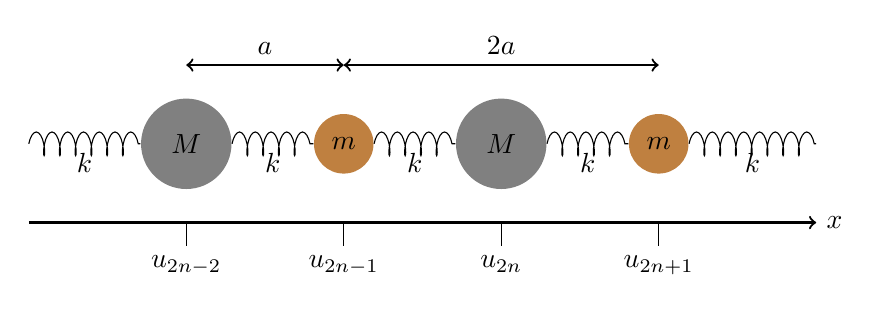
\begin{tikzpicture}
    \node[circle,fill=gray,inner sep=2.5mm] (a1) at (2,0){$M$};
    \node[circle,fill=brown,inner sep=1.5mm] (b1) at (4,0){$m$};
    \node[circle,fill=gray,inner sep=2.5mm] (a2) at (6,0){$M$};
    \node[circle,fill=brown,inner sep=1.5mm] (b2) at (8,0){$m$};
    \draw[decoration={aspect=0.3, segment length=2mm, amplitude=1.5mm,coil},decorate](0,0)--(a1) node[midway,below]{$k$};
    \draw[decoration={aspect=0.3, segment length=2mm, amplitude=1.5mm,coil},decorate](a1)--(b1)node[midway,below]{$k$};
    \draw[decoration={aspect=0.3, segment length=2mm, amplitude=1.5mm,coil},decorate](b1)--(a2)node[midway,below]{$k$};
    \draw[decoration={aspect=0.3, segment length=2mm, amplitude=1.5mm,coil},decorate](a2)--(b2)node[midway,below]{$k$};
    \draw[decoration={aspect=0.3, segment length=2mm, amplitude=1.5mm,coil},decorate](b2)--(10,0)node[midway,below]{$k$};
    \draw[->,thick](0,-1)--(10,-1) node[right]{$x$};
    \draw (2,-1)--(2,-1.3) node[anchor=north]{$u_{2n-2}$};
    \draw (4,-1)--(4,-1.3) node[anchor=north]{$u_{2n-1}$};
    \draw (6,-1)--(6,-1.3) node[anchor=north]{$u_{2n}$};
    \draw (8,-1)--(8,-1.3) node[anchor=north]{$u_{2n+1}$};
    \draw [<->,thick](2,1)--(4,1) node[midway,above]{$a$};
    \draw [<->,thick](4,1)--(8,1) node[midway,above]{$2a$};
\end{tikzpicture}
\caption{1维双原子链}
\end{figure}

考虑简谐近似,设谐振子的劲度系数为\emph{k},设一个原子质量为M,另一原子质量为m,相邻原子间距\emph{a},
相邻同质量原子的间距为\emph{2a},因此方程写为:
\begin{equation*}
    \left\{\begin{aligned}
        M\ddot{u}_{2n}&=k(u_{2n+1}-u_{2n})-k(u_{2n}-u_{2n-1})\\
        m\ddot{u}_{2n-1}&=k(u_{2n}-u_{2n-1})-k(u_{2n-1}-u_{2n-2}) 
    \end{aligned}\right.
\end{equation*}
由于相邻的同类原子间距为\emph{2a},考虑行波解:
$$u_{2n}=Ae^{i(qn2a-\omega t)},\ \ \ \ u_{2n-1}=Be^{i(qn2a-\omega t)}$$
代入方程后,化简得:
\begin{equation*}
    \left\{\begin{aligned}
        (M\omega^2-2k)A+k(e^{iq2a}+1)B&=0\\
        k(e^{-iq2a}+1)A+(m\omega^2-2k)B&=0
    \end{aligned}\right.
\end{equation*}
要求A,B有非零解,即要求系数行列式为0,解方程:
\begin{equation*}
    \left|\begin{array}{ccc}
        M\omega^2-2k & k(e^{iq2a}+1)\\
        k(e^{-iq2a}+1) & m\omega^2-2k
    \end{array}\right|=0
\end{equation*}
解得两支色散关系为:
\begin{equation*}
    \left\{\begin{aligned}
        \omega_A^2&=\frac{k}{Mm}\left[(M+m)-\sqrt{(M+m)^2-4Mm\sin^2{qa}}\right]\\
        \omega_O^2&=\frac{k}{Mm}\left[(M+m)+\sqrt{(M+m)^2-4Mm\sin^2{qa}}\right]
    \end{aligned}\right.
\end{equation*}
考虑当$M=m$的情形,上式简化为:
\begin{equation*}
    \left\{\begin{aligned}
        \omega_A^2&=\frac{2k}{m}\left(1-\cos{qa}\right)\\
        \omega_O^2&=\frac{2k}{m}\left(1+\cos{qa}\right)
    \end{aligned}\right.
\end{equation*}
可以看到,由于$-1\leq\cos{qa}\leq 1$,因此光学支和声学支在这里的取值实际上是一致的,都符合一维晶格振动值,但相位恰好相差$\pi$.这种相位差产生的原因是布里渊区折叠,即在
取晶格常数时计算取值比实际晶格常数大一倍,于是布里渊区的线度缩小一倍,光学支和声学支发生一个$\pi$的相位差.
\vskip 0.5cm
\section*{习题2}
考虑一个全同的原子组成的平面正方格子,用$u_{l,m}$表示第\emph{l}行第\emph{m}列的原子在垂直于与晶格平面方向的位移,每个原子质量为\emph{M},最近邻原子之间的
距离为\emph{a},只考虑最近原子之间的相互作用,最近邻原子在垂直于晶格平面方向上的力常数为$\beta$,
\begin{itemize}
    \item[(1).]试求原子在垂直于晶体平面方向的振动方程.
    \item[(2).]设该振动方程的行波解的形式为:$$u_{l,m}=u_0 e^{i(k_xla+k_yma-\omega t)}$$试求出其色散关系.
    \item[(3).]证明独立的行波解存在的\emph{k}空间区域是一个边长为$\frac{2\pi}{a}$的正方形,画出$k=k_x,\ k_y=0$,以及$k=k_x=k_y$时的色散关系.
    \item[(4).]对于$k_xa\ll 1,\ k_ya\ll 1$,求出长波近似下的色散关系.    
\end{itemize}
\vskip 0.3cm
\noindent{\heiti{解}}:

\noindent (1).考虑第(\emph{l,m})个原子的位移为$u_{l,m}$,则振动方程是:
$$M\ddot{u}_{l,m}=\beta(u_{l+1,m}+u_{l-1,m}+u_{l,m+1}+u_{l,m-1}-4u_{l,m})$$

\noindent (2).将行波解$u_{l,m}=u_0 e^{i(k_xla+k_yma-\omega t)}$代入振动方程中,考虑:
\begin{gather*}
    u_{l+1,m}=e^{ik_xa}u_{l,m},\ \ \ \ u_{l-1,m}=e^{-ik_xa}u_{l,m}\\
    u_{l,m+1}=e^{ik_ya}u_{l,m},\ \ \ \ u_{l,m-1}=e^{-ik_ya}u_{l,m}
\end{gather*}
代入方程求解,有色散关系:
$$\omega^2=\frac{2\beta(2-\cos{k_xa}-\cos{k_ya})}{M}$$

\noindent (3).将波矢数限制在一个周期内$\omega\left(\vec{q}+\frac{2\pi}{a}(\vec{i}+\vec{j})\right)=\omega(\vec{q})$容易得到:
$$-\frac{\pi}{a}\leq k_x\leq\frac{\pi}{a},\ \ \ \ -\frac{\pi}{a}\leq k_y\leq\frac{\pi}{a}$$
当$k=k_x,\ k_y=0$时,色散关系:$\omega^2=\frac{4\beta}{M}\sin^2{\frac{ka}{2}}$,图像为:
\begin{figure}[h]
	\centering
	\begin{tikzpicture}[global scale = 1]
	\coordinate (O) at (0,0);
	\coordinate (A) at (-pi,0);
    \coordinate (B) at (pi,0);
    \coordinate (C) at (0,4);
	\draw[->](-3.5,0)--(3.5,0)node[left,below,font=\tiny]{$k$};
	\draw[->](0,-0.2)--(0,4.2)node[right,font=\tiny]{$\omega$};
	\draw[dashed](-3.5,4)--(3.5,4);
	\draw[dashed](-pi,0)--(-pi,4.2);
	\draw[dashed](pi,0)--(pi,4.2);
	\draw (A) node[below] {$-\frac{\pi}{a}$} -- ++(0, 3pt);
    \draw (B) node[below] {$\frac{\pi}{a}$} -- ++(0, 3pt);
    \draw (C) node[left] {$\sqrt{\frac{4\beta}{M}}$} -- ++(0, 3pt);
    \draw (O) node[below] {$O$};
    \draw[domain = 0:pi, smooth] plot(\x,{4*sin((1/2)*\x r)});
    \draw[domain = -pi:0, smooth] plot(\x,{-4*sin((1/2)*\x r)});
	\end{tikzpicture}
	\caption{$k_x=k,\ k_y=0$时色散关系图像}
	\end{figure}

当$k=k_x=k_y$时,色散关系:$\omega^2=\frac{8\beta}{M}\sin^2{\frac{ka}{2}}$,图像为:
\begin{figure}[h]
	\centering
	\begin{tikzpicture}[global scale = 1]
	\coordinate (O) at (0,0);
	\coordinate (A) at (-pi,0);
    \coordinate (B) at (pi,0);
    \coordinate (C) at (0,4);
	\draw[->](-3.5,0)--(3.5,0)node[left,below,font=\tiny]{$k$};
	\draw[->](0,-0.2)--(0,4.2)node[right,font=\tiny]{$\omega$};
	\draw[dashed](-3.5,4)--(3.5,4);
	\draw[dashed](-pi,0)--(-pi,4.2);
	\draw[dashed](pi,0)--(pi,4.2);
	\draw (A) node[below] {$-\frac{\pi}{a}$} -- ++(0, 3pt);
    \draw (B) node[below] {$\frac{\pi}{a}$} -- ++(0, 3pt);
    \draw (C) node[left] {$\sqrt{\frac{8\beta}{M}}$} -- ++(0, 3pt);
    \draw (O) node[below] {$O$};
    \draw[domain = 0:pi, smooth] plot(\x,{4*sin((1/2)*\x r)});
    \draw[domain = -pi:0, smooth] plot(\x,{-4*sin((1/2)*\x r)});
	\end{tikzpicture}
	\caption{$k_x=k_y=k$时色散关系图像}
	\end{figure}

\noindent (4).对于$k_xa\ll 1,\ k_ya\ll 1$,小量展开保留到二阶项:
$$\omega^2\approx\frac{2\beta}{M}\left[2-\left(1-\frac{(k_xa)^2}{2}\right)-\left(1-\frac{(k_ya)^2}{2}\right)\right]=\frac{\beta}{M}\left[(k_xa)^2+(k_ya)^2\right]$$
\vskip 0.5cm
\section*{习题3}
试从黄昆方程出发证明LST关系,即:$\frac{\omega_{LO}^2}{\omega_{TO}^2}=\frac{\varepsilon(0)}{\varepsilon(\infty)}$.
\vskip 0.3cm
\noindent{\heiti{证}}:

考虑到$\overrightarrow{W},\ \overrightarrow{E},\ \overrightarrow{P}$写成纵波和横波的形式.
$$
\overrightarrow{W}=\overrightarrow{W_L}+\overrightarrow{W_T}
$$
$$
\overrightarrow{P}=\overrightarrow{P_L}+\overrightarrow{P_T}
$$
$$
\overrightarrow{E}=\overrightarrow{E_L}+\overrightarrow{E_T}
$$
对于纵波,其振动方向平行于波矢方向,因此纵波分量的旋度为0,即:
$$\nabla\times\overrightarrow{W_L}=\nabla\times\overrightarrow{P_L}=\nabla\times\overrightarrow{E_L}=0$$
对于横波,其振动方向垂直于波矢方向,因此横波分量的散度为0,即:
$$\nabla\cdot\overrightarrow{W_T}=\nabla\cdot\overrightarrow{P_T}=\nabla\cdot\overrightarrow{E_T}=0$$
带入黄昆方程,写成分量形式有:
\begin{equation*}
    \left\{\begin{aligned}
        \ddot{\ora{W_T}}=b_{11}\ora{W_T}+b_{12}\ora{E_T}\\
        \ddot{\ora{W_L}}=b_{11}\ora{W_L}+b_{12}\ora{E_L}
    \end{aligned}\right.
\end{equation*}
对于横波,考虑Maxwell方程组,在无外加磁场的情况下,即:$\ora{B}=0$,于是有$\nabla\times\ora{E}=0$,有:
$$\nabla\times\ora{E}=\nabla\times(\ora{E_T}+\ora{E_L})=\nabla\times\ora{E_T}=0$$
又因为:$\nabla\cdot\ora{E_T}=0$,因此$\ora{E_T}$是一个常矢量.
$\because\omega_0^2=-b_{11},\ \therefore\omega_{TO}=\omega_{0}$

对于纵波,考虑Maxwell方程组,由于无自由电荷密度,故$\nabla\cdot\ora{D}=0$,于是:
$$\nabla\cdot\ora{D}=\nabla\cdot(\ora{E}+4\pi\ora{P})=\nabla\cdot(\ora{E_T}+\ora{E_L}+4\pi\ora{P_T}+4\pi\ora{P_L})=\nabla\cdot(\ora{E_L}+4\pi\ora{P_L})=0$$
$\because\nabla\times(\ora{E_L}+4\pi\ora{P_L})=0$,因此$\ora{E_L}+4\pi\ora{P_L}$是一个常矢量.
考虑黄昆方程:
$$\ora{P_L}=b_{12}\ora{W_L}+b_{22}\ora{E_L}$$
有
$$\ora{E_L}=-\frac{4\pi b_{12}}{1+4\pi b_{22}}\ora{W_L}$$
联立黄昆方程第一项方程,得到:
$$\ddot{\ora{W_L}}=(b_{11}-\frac{4\pi b_{12}}{1+4\pi b_{22}})\ora{W_L}=-\omega_{LO}^2\ora{W_L}$$
考虑到:
$$\varepsilon(\omega)=1+4\pi(b_{22}-\frac{b_{12}^2}{b_{11}+\omega^2})$$
取短波情况和长波情况,有:
$$\varepsilon(0)\approx 1+4\pi(b_{22}+\frac{b_{12}^2}{\omega_0^2}),\ \ \ \varepsilon(\infty)\approx 1+4\pi b_{22}$$
联立有:
$$b_{12}=\sqrt{\frac{\varepsilon(0)-\varepsilon(\infty)}{4\pi}}\omega_{TO},\ \ \ b_{22}=\frac{\varepsilon(\infty)-1}{4\pi}$$
于是有:
$$\frac{\omega_{LO}^2}{\omega_{TO}^2}=\frac{\varepsilon(0)}{\varepsilon(\infty)}$$
证毕.
\vskip 0.5cm
\section*{习题4}
试求一维单原子晶格振动的模式密度$D(\omega)$.
\vskip 0.3cm
\noindent{\heiti{解}}:

一维原子链的波矢密度为:$\frac{L_c}{2\pi}\dd q$

由于$\omega(-q)=\omega(q)$,频率$\dd\omega$内的振动模式数:$\delta n=2\times\frac{L_c}{2\pi}\frac{\dd q}{\dd\omega}\dd\omega$

考虑色散关系
$$\omega=2\left(\frac{\beta}{m}\right)^{\frac{1}{2}}\sin{\left(\frac{qa}{2}\right)}$$

故振动模式为:
$$D(\omega)=\frac{L_c}{\pi}\frac{1}{\frac{\dd\omega}{\dd q}}=\frac{2L_c}{a\pi\sqrt{\omega_0^2-\omega^2}}$$

\vskip 0.5cm
\section*{习题5}
对于三维晶格的光学振动在长波极限下的色散关系为:$$\omega(q)=\omega_0-Aq^2$$证明:相应的晶格振动的模式密度为:
\begin{equation*}
    D(\omega)=\left\{\begin{aligned}
        \frac{V_c}{4\pi^2}A^{-\frac{3}{2}}&(\omega_0-\omega)^{-\frac{1}{2}},\ \ &\omega<\omega_0\\
        &0,&\omega>\omega_0
    \end{aligned}\right.
\end{equation*}
\vskip 0.3cm
\noindent{\heiti{证}}:

考虑三维晶体中第$\alpha$支格波的模式密度计算式:
$$D(\omega)=\frac{V_c}{(2\pi)^3}\int_{S_{\alpha}}{\frac{\dd S}{|\nabla_q \omega|}}$$
$S_{\alpha}$是第$\alpha$支格波的等频面,考虑光学支在长波近似的极限情况下,等频面是一个球面。
考虑这里的色散关系:$\omega(q)=\omega_0-Aq^2$,于是有:$|\nabla_q\omega|=2Aq$,则:
$$D(\omega)=\frac{V_c}{(2\pi)^3}\frac{1}{2Aq}\int_{S_{\alpha}}{\dd S}=\frac{V_c}{(2\pi)^3}\frac{4\pi q^2}{2Aq}=\frac{V_c(\omega_0-\omega)^{\frac{1}{2}}}{4A^{\frac{3}{2}}\pi^2}$$
其中$q=\sqrt{\frac{\omega_0-\omega}{A}}$,于是上式成立的条件是$\omega_0>\omega$.

对于$\omega>\omega_0$的情况,发现$q^2=\frac{\omega_0-\omega}{A}$,也就是这个色散关系下为复数波矢,这种情况下,近似不再适用,于是有:
\begin{equation*}
    D(\omega)=\left\{\begin{aligned}
        \frac{V_c}{4\pi^2}A^{-\frac{3}{2}}&(\omega_0-\omega)^{-\frac{1}{2}},\ \ &\omega<\omega_0\\
        &0,&\omega>\omega_0
    \end{aligned}\right.
\end{equation*}
\vskip 0.5cm
\section*{习题6}
有N个相同的原子组成的面积为S的二维晶格。试在德拜模型下计算:
\begin{itemize}
    \item[(1).]晶格振动的比热,并论述在低温极限下比热与温度的关系.
    \item[(2).]平均声子数目,并论述在低温极限下平均声子数与温度的关系.  
\end{itemize}
\vskip 0.3cm
\noindent{\heiti{解}}:

\noindent (1).二维格子的声子态密度为:$D(\omega)=\frac{S_c}{\pi v_p^2}\omega$
其中:$\frac{1}{v_p^2}=\frac{1}{v_L^2}+\frac{1}{v_T^2}$
考虑简单格子有N个原子,振动模式为2N,且全为声学支振动.则:
$$\int_{\omega_{min}}^{\omega_{max}}{D(\omega)\dd\omega}=2N$$
由于声学支色散关系:$\omega=vq$,长波近似下$q\to 0$,故$\omega_{min}\to 0$.
设$\omega_{max}=\omega_D$,则根据积分式得到:
$$\omega_D=\sqrt{\frac{4\pi N}{S_c}}v_p$$
计算热容为:
$$C_V=k_B\frac{S_c}{\pi v_p^2}\int_{0}^{\omega_D}{\frac{\left(\frac{\hbar\omega}{k_BT}\right)^2 e^{\frac{\hbar\omega}{k_BT}}}{\left(e^{\frac{\hbar}{k_BT}}-1\right)^2}\omega\dd\omega}$$
作变量代换$x=\frac{\hbar\omega}{k_BT}$,有$\Theta_D=\frac{\hbar\omega_D}{k_B}$,于是:
$$C_V=\frac{S_ck_B}{\pi v_p^2}\left(\frac{k_BT}{\hbar}\right)^2\int_{0}^{\frac{\Theta_D}{T}}{\frac{e^xx^3}{(e^x-1)^2}\dd x}$$
低温近似下,有$\frac{\Theta_D}{T}\to\infty$,积分:
$$\int_{0}^{\infty}{\frac{e^xx^3}{(e^x-1)^2}\dd x}$$
可以计算出,结果由$\zeta$函数表示,于是:
$$C_V=\frac{6\zeta(3)S_ck_B^3}{\pi v_p^2\hbar^2}T^2$$
即:极低温度下热容与温度的二次方成正比.

\noindent (2).平均声子数目:
$$\overline{N}=\frac{S_c}{\pi v_p^2}\int_{0}^{\omega_D}{\frac{\omega\dd\omega}{e^{\frac{\hbar\omega}{k_BT}}-1}}$$
作变量代换$x=\frac{\hbar\omega}{k_BT}$,得:
$$\overline{N}=\frac{4NT^2}{\Theta_D}\int_{0}^{\frac{\Theta_D}{T}}{\frac{x\dd x}{e^x-1}}$$
在极低温度下,有$\frac{\Theta_D}{T}\to\infty$,于是:
$$\overline{N}=\frac{2\pi NT^2}{3\Theta}$$
\end{document}